%!TEX root = ../thesis.tex
% chapter 3

\chapter{Strongly coupled plasma}
\label{sec:ch3}

The plasma in which the Coulomb potential energy of the system exceeds the thermal kinetic energy of the particles is called the strongly coupled plasma (SCP). The Coulomb coupling parameter of plasma is defined as
\begin{equation}
\begin{aligned}
\Gamma &= \frac{U}{K}=\frac{e^{2} / 4 \pi \varepsilon_{0} R_\text{WS}}{k_\text{B} T_{e}} \\
&=\left(\frac{e^{2}}{4 \pi \varepsilon_{0} k_\text{B} T_{e}}\right)\left(\frac{4 \pi n_{e}}{3}\right)^{1 / 3}
\end{aligned}
\end{equation}
, where $U$ and $K$ are average coulomb potential and kinetic energy of an electron, and $e$, $\varepsilon_0$, $k_\text{B}$, $R_\text{WS}$, $T_e$, and $n_e$ are electron charge, vacuum permeability, Boltzmann constant, Wigner-Seitz radius, electron temperature and electron density, respectively. Technically SCP satisfy $\Gamma \geq 1$. Standard theories for an ideal plasma fail to describe such conditions of strongly correlated systems \cite{stanton2016ionic}. The SCPs are found in many objects such as stars, galaxies, white dwarf stars, cores of Jovian planets \cite{ichimaru1982strongly}, lightening in the thick planetary atmospheres \cite{cartier2020planetary}, and inertial confinement fusion \cite{remington2006experimental}, bringing both scientific and technical interests. Owing to their theoretical and practical importance, a great amount of effort was dedicated for a few decades.



%----------------------------------------------------------------------------------------------------
\section{Physical regimes}
\label{sec:ch3-1}

The plasmas can be classified within the phase diagram consisting of temperature and density of electrons. Strongly coupled dense plasmas span a wide range of unfamiliar regimes having high density and relatively low temperature (Fig.\ref{fig:taxonomy}). Due to the close proximity of ions, SCP exhibits the features of condensed matter. Both theories on classical (ideal) plasma physics and condensed matter (quantum) physics are required to understand such plasmas. In addition to the coupling parameter $\Gamma$, there are several more parameters for defining which region the plasma corresponds to and what kind of theories should be applied according to the electron temperature and density, such as Debye number $N_\text{D}$, energy density $P$, and degeneracy parameter $\Theta$.

%----------
\subsection{Assumptions for ideal plasma}
\label{sec:ch3-1-1}

For an ideal plasma, the Debye length $\lambda_\text{D}$ is the nominal shielding length of a charged particle. A particle outside the Debye sphere with a radius of Debye length does not ``feel'' the Coulomb potential. The Debye number $N_\text{D}$ is the number of electrons in the Debye sphere. The concept of Debye shielding is achieved from a circular logic for an ideal plasma. The two assumptions that the collisions between particles are negligible and that $N_\text{D}$ is sufficiently large guarantee each other, and only, in that case, the Debye shielding is valid \cite{bellan2008fundamentals}.

\begin{figure}[ht!]
\centering
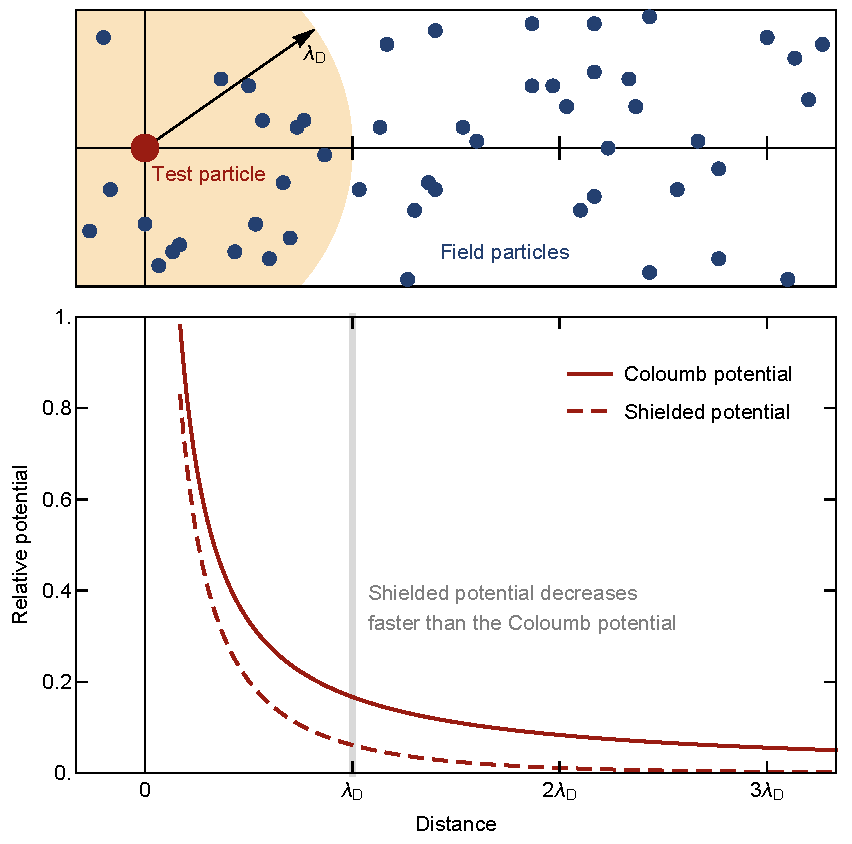
\includegraphics[width=100mm]{figures/ch3/Debye/shielding.pdf}
\caption{Schematic diagram for the Debye shielding. As the charge of the test particle is gradually introduced, the surrounding field particles move to cancel out the electrostatic potential.}
\label{fig:DebyeShielding}
\end{figure}

The Debye length is obtained from the following three relations: Boltzmann relation, Poisson equation, and charge neutrality. First, let us consider the Boltzmann relation starting with the equation of motion for each species s
\begin{equation}
m_\text{s} \frac{d \vec{v}_\text{s}}{d t} = -q_\text{s} \nabla \phi - \frac{\nabla  p_\text{s}}{n_\text{s}}
\label{eq:EOM}
\end{equation}
, where $\vec{v}_\text{s}$ and $p_\text{s}$ are the velocity and pressure for the species s. The omitted terms in the above equation are as follows: 1. the Lorentz force $q \vec{v} \cross \vec{B}$, 2. vector potential in the electric field $\vec{E} = -\nabla \phi - \partial \vec{A} / \partial t$, 3. collision (friction) force $\vec{R}_f$, and 4. viscosity. What assumptions make it possible to exclude these terms? There are four assumptions: 1. negligible magnetic field ($q \vec{v} \cross \vec{B} \approx 0$), 2. slow transition ($\partial \vec{A} / \partial t \approx 0$), 3. collisionless plasma (no friction and no viscosity), and 4. well defined temperature (the particle for each species are in thermal equilibrium among themselves and their energy distribution follows the Maxwellian distribution function). The pressure gradient term is approximated as 
\begin{equation}
\begin{aligned}
\nabla p_\text{s} &= k_\text{B} T_\text{s} \nabla n_\text{s} + n_\text{s} \nabla \left( k_\text{B} T_\text{s} \right) \\
&= k_\text{B} T_\text{s} n_\text{s} \left( \frac{\nabla n_\text{x}}{n_\text{s}} + \frac{\nabla T_\text{s}}{T_\text{s}} \right) \\
&\approx k_\text{B} T_\text{s} \nabla n_\text{s}
\end{aligned}
\end{equation}
, when $\nabla n/n \gg \nabla T/T$ by assuming the temperature gradient is very small. From the slow transition approximation, the Eq.\ref{eq:EOM} becomes
\begin{equation}
- q_\text{s} \nabla \phi - \left( \frac{k_\text{B} T_\text{s} \nabla n_\text{s}}{n_\text{s}} \right) \approx 0
\end{equation}
When $\phi \left( \vec{r} \right)$ and $T_\text{s} \left( \vec{r} \right)$ are spatially uniform, we get the Boltzmann relation
\begin{equation}
n_\text{s} \left(\vec{r} ~\right) = n_\text{s0} \left( \vec{r} ~\right) \exp \left[ \frac{-q_\text{s} \phi \left( \vec{r} ~\right)}{k_\text{B} T_\text{s} \left( \vec{r} ~\right) }\right]
\label{eq:BoltzmannRelation}
\end{equation}
If the potential energy is much smaller than the kinetic energy, i.e. $\abs{q_\text{s} \phi / k_\text{B} T}\ll 1$, the Eq.\ref{eq:BoltzmannRelation} simplifies to 
\begin{equation}
n_\text{s} \left(\vec{r} ~\right) \approx n_\text{s0} \left( \vec{r} ~\right) \left[ 1- \frac{q_\text{s} \phi \left( \vec{r} ~\right)}{k_\text{B} T_\text{s} \left( \vec{r} ~\right) }\right]
\label{eq:BoltzmannRelationApprox}
\end{equation}
The relations to consider next are the Poisson equation and the charge neutrality:
\begin{equation}
\begin{aligned}
\nabla \cdot \vec{E} &= - \nabla^2 \phi \\
&= \frac{\rho}{\varepsilon_0} \\
&= \frac{q_\text{T} \delta \left( \vec{r} ~\right) +\sum_\text{s} q_\text{s} n_\text{s} \left( \vec{r} ~\right)}{\varepsilon_0}
\end{aligned}
\label{eq:Poisson}
\end{equation}
\begin{equation}
\sum_\text{s} q_\text{s} n_\text{s,o} = 0
\label{eq:chargeNeutral}
\end{equation}
, where $q_\text{T}$ is the charge of the test particle and $\rho$ is the total charge density.
By plugging the Eq.\ref{eq:BoltzmannRelationApprox} and \ref{eq:chargeNeutral} into the \ref{eq:Poisson}, we get
\begin{equation}
- \nabla^2 \phi = \frac{q_\text{T}}{\varepsilon_0} \delta \left( \vec{r} ~\right) - \sum_\text{s} \left( \frac{n_\text{s0} q_\text{s}^2}{\varepsilon_0 k_\text{B} T_\text{s}} \right) \phi
\label{eq:PoissonApprox}
\end{equation}
Let us define the Debye length $\lambda_\text{s}$ of each species s as
\begin{equation}
\frac{1}{\lambda_\text{s}^2} \equiv \frac{n_\text{s0} q_\text{s}^2}{\varepsilon_0 k_\text{B} T_\text{s}}
\end{equation}
and the total Debye length $\lambda_\text{D}$ writes
\begin{equation}
\frac{1}{\lambda_\text{D}} \equiv \sum_\text{s} \left( \frac{1}{\lambda_\text{s}^2} \right)
\end{equation}
Now Eq.\ref{eq:PoissonApprox} becomes
\begin{equation}
- \nabla^2 \phi + \frac{1}{\lambda_\text{D}^2} \phi = \frac{q_\text{T}}{\varepsilon_0} \delta \left( \vec{r} ~\right)
\label{eq:PoissonApproxSimplified}
\end{equation}
Finding the spherically symmetric solution of the form
\begin{equation}
\phi=\frac{f(r) q_\text{T}}{4 \pi \epsilon_{0} r}
\end{equation}
, and note that the delta function writes 
\begin{equation}
\nabla^{2}\left(\frac{1}{r}\right)=-4 \pi \delta \left( \vec{r} \right)
\end{equation}
We get $f(0)=1$ and $f''(r)=f(r)/\lambda_\text{D}^2$ which leads the final solution 
\begin{equation}
\phi \left( \vec{r} ~\right) = \frac{q_\text{T}}{4 \pi \varepsilon_0 r} \exp \left( -\frac{r}{\lambda_\text{D}} \right)
\label{eq:shieldedPotential}
\end{equation}

The potential of the form of Eq.\ref{eq:shieldedPotential} is called in several names such as Yukawa potential, Debye-H\"{u}kel potential, or shielded Coulomb potential. Recalling that any particle could have been the test particle, the effective potential of any plasma particle is described with the Eq.\ref{eq:shieldedPotential}. Note that, this analysis is only valid when the number of charged particle within the shielding sphere with a radius $\lambda_\text{D}$ (called Debye number $N_\text{D}$) is large enough, i.e. $N_\text{D} = 4 \pi n_0 \lambda_\text{D}^3/3 \gg 1$. To conclude, the Debye shielding and the collisionless nature are the interdependent conditions for the ideal plasmas, both of which are valid only when the Debye number is large enough.

%----------
\subsection{Failure of Debye shielding}
\label{sec:ch3-1-2}

In the case of SCP with high electron density, the screening is not possible because the distance among the particles is small compared to the Debye length. If the Debye shielding concept predicted from the ideal plasma theory is simply expanded, we encounter $N_\text{D} < 1$ at some point. As discussed above, Debye shielding is only valid when a sufficient number of charged particles are guaranteed to exist.

\begin{figure}[ht!]
\centering
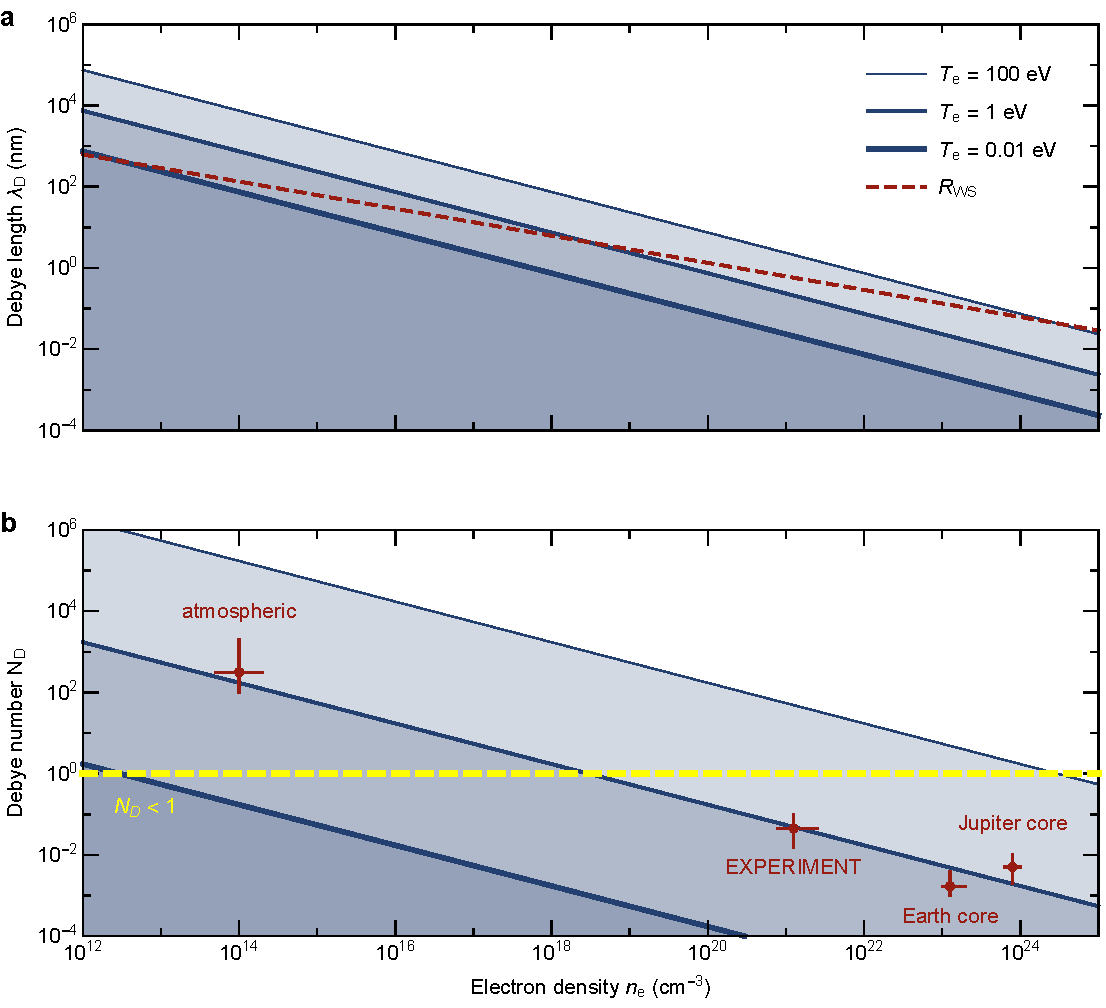
\includegraphics[width=130mm]{figures/ch3/Debye/number.pdf}
\caption{Straightforward extension of Debye shielding concept to a dense plasma. \textbf{a,} When the electron density increases, at some point, the inter-particle distance exceeds the Debye length. \textbf{b,} The Debye number drops below unity, and the shielding assumption does not hold anymore. The cores of planets, as well as the plasma generated in our experiment, are under such conditions.}
\label{fig:DebyeNumber}
\end{figure}

\begin{figure}[ht!]
\centering
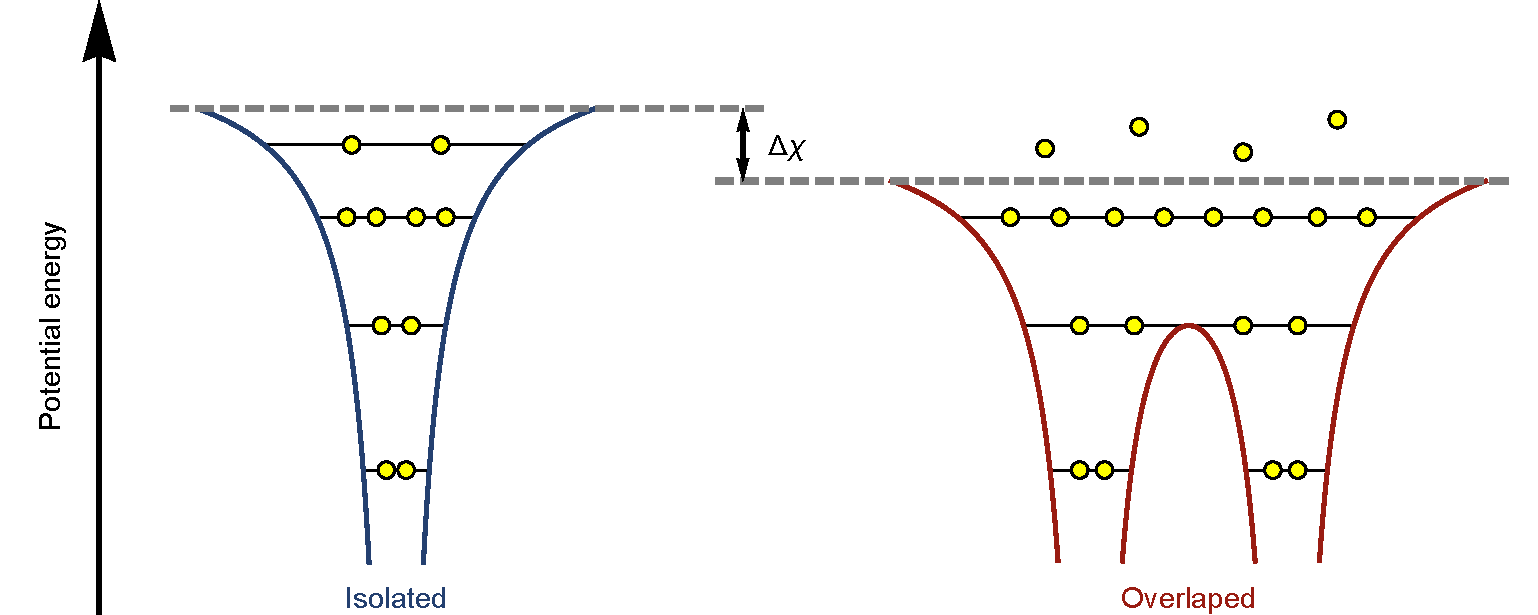
\includegraphics[width=130mm]{figures/ch3/lowering/continuumLowering.pdf}
\caption{Graphical illustration of continuum lowering. When atoms are close together, the energy levels are distorted by adjacent neighbors, and the valence electrons do not stay in the bound levels anymore.}
\label{fig:continuumLowering}
\end{figure}

When the Debye shielding is not valid, the energy levels of atoms are distorted by adjacent neighbors, and the valence electrons may be released from the atoms (Fig.\ref{fig:continuumLowering}). This phenomenon is called continuum lowering, and the plasma exhibits the features of liquid metal or condensed matter. The amount of continuum lowering for the strongly coupled plasma is \cite{griem1962high, bataller2014blackbody}
\begin{equation}
\Delta \chi = \frac{(\bar{Z}+1) e^{3}}{4 \pi \varepsilon_{0}} \sqrt{\frac{\bar{Z}(\bar{Z}+1) n_{0}}{\varepsilon_{0} k_{B} T_{e}}}
\label{eq:lowering}
\end{equation}
, where $\bar{Z}$ is the effective degree of ionization, $e$ is the electron charge, and $\varepsilon_0$ is the vacuum permittivity \cite{bataller2014blackbody, griem1962high}.

In such plasma, the electrons become degenerate as the Pauli exclusion principle comes in for the occupation of the free electron states, and they start to follow Fermi-Dirac statistics \cite{murillo2004strongly}. The degeneracy parameter gives a measure of the importance of degeneracy,
\begin{equation}
\Theta=\frac{T_{e}}{T_{F}}=\frac{2 m_{e} k_{B} T_{e}}{\hbar^{2}\left(3 \pi^{2} n_{e}\right)^{2 / 3}}
\end{equation}
, where $T_\text{F}$ is the Fermi temperature.
The regime corresponding to $\Theta \leq 1$ is shown as a shaded area with dark-red color on the top-left corner of Fig.\ref{fig:taxonomy}. When $\Theta \gg 1$, the electrons are considered to follow the classical Maxwell-Boltzmann statistics, and, in the other case, they follow Fermi-Dirac statistics.



%----------------------------------------------------------------------------------------------------
\section{Electron-ion collision}
\label{sec:ch3-2}

The energy relaxation from electron to ion is governed by
\begin{equation}
\frac{d \mathcal{E}_e}{d t}=-\nu_{Eei}\left(\mathcal{E}_{e}-\mathcal{E}_{i}\right)
\end{equation}
, where $\mathcal{E}_{e(i)}$ is the electron (ion) energy, and $\nu_{Eei}$ is the collision frequency of energy change from electron to ion. Note that, as the ion to electron mass ratio is very large, the orders of momentum or energy collision frequency between species are diverse (see Table.\ref{table:collFreq}). In this case, $\nu_{Eei} = \left( m_e/m_i \right) \nu_{ei}$.

\begin{table}[h!]
\footnotesize
\centering
\begin{tabular}{ccc}
\hline \hline
$\sim 1$        &   $\sim \left( m_e/m_i \right)^{1/2}$   &   $\sim m_e/m_i$   \\ \hline
$\nu_{ee}$     &   $\nu_{ii}$                                        &   $\nu_{ie}$             \\
$\nu_{ei}$      &   $\nu_{Eii}$                                      &   $\nu_{Eei}$           \\
$\nu_{Eee}$   &                                                          &   $\nu_{Eie}$            \\
\hline \hline
\end{tabular}
\caption{The orders of momentum or energy collision frequencies between electron between species \cite{bellan2008fundamentals}. The energy transfer frequency from electron to ion $\nu_{Eei}$ is smaller from momentum transfer frequency $\nu_{ei}$ by the mass ratio of electron to ion.}
\label{table:collFreq}
\end{table}

For a weakly coupled ideal plasma, most theories obtain the energy relaxation rate from electron to ion as
\begin{equation}
\nu_{ei}=\frac{8}{3} n_{i} \left( \frac{Z e^{2}}{4\pi \varepsilon_0} \right)^2 \left( \frac{m_i}{m_e} \right) \frac{\sqrt{2 \pi m_e m_i}}{\left(m_e k_{B} T_{i} + m_i k_{B} T_{e}\right)^{3 / 2}} \ln{\Lambda}
\end{equation}
, where $\ln{\Lambda}$ is called Coulomb logarithm \cite{dimonte2008molecular}. For the typical conditions of $m_e \ll m_i$ and $T_e \sim T_i$,
\begin{equation}
\nu_{ei} = \frac{1}{3} \sqrt{\frac{8}{\pi}} \left( \frac{R_c}{\lambda_\text{D}} \right) \omega_{pe} \ln{\Lambda}
\end{equation}
, where $R_c \equiv Z e^2/k_\text{B} T_e $ is Landau length which represents the smallest relevant impact parameter and $\omega_{pe} = \sqrt{n_{e} e^{2} / \varepsilon_0 m_e}$ is the plasma frequency. The above equation can be expressed in terms of coupling parameter $\Gamma$ as
\begin{equation}
\nu_{ei} = \sqrt{\frac{8}{3\pi}} \omega_{pe} \Gamma^{3/2} \ln{\Lambda}
\end{equation}
The Coulomb logarithm for an ideal plasma is in the form $\ln{\Lambda} = \ln{\left( C/g \right)}$, where $g \equiv R_c/\lambda_\text{D}$, and the numerical constant $C$ ranges from $1 \sim 3$, which leads
\begin{equation}
\nu_{ei} = \sqrt{\frac{8}{3\pi}} \omega_{pe} \Gamma^{3/2} \ln{\left( \frac{C}{g} \right)}
\end{equation}

For the case of an SCP, the above collision frequency writes 
\begin{equation}
\nu_{ei} = \frac{2}{\sqrt{6\pi}} \omega_{pe} \Gamma^{3/2} \ln{ \left( 1+ \frac{0.7}{g} \right)}
\end{equation}
with further modification in the Coulomb logarithm \cite{dimonte2008molecular, bataller2014blackbody, zel2002physics}.

If the plasma is dense and opaque, the collisionality is, once again, modified under the presence of an oscillating electromagnetic field of frequency $\omega$, and the momentum collision frequency becomes
\begin{equation}
\nu_{ei} = \frac{2}{\sqrt{6\pi}} \omega_{pe} \Gamma^{1/2} \Gamma_\omega \ln{ \left( 1+ \frac{0.7}{g} \right)}
\end{equation}
, where $\Gamma_\omega$ is the plasma coupling parameter under the presence of an electromagnetic field which is tweaked in the way of appending a transcendental function as follows:
\begin{equation}
\Gamma_{\omega}=\Gamma\left[\frac{k_{B} T_e}{\hbar \omega}\left(1-\exp \left(-\frac{\hbar \omega}{k_{B} T_e}\right)\right)\right]
\end{equation}
The coupling parameter $\Gamma_\omega$ decreases when the electron temperature is smaller than the photon energy (Fig.\ref{fig:modifiedGamma}).

\begin{figure}[ht!]
\centering
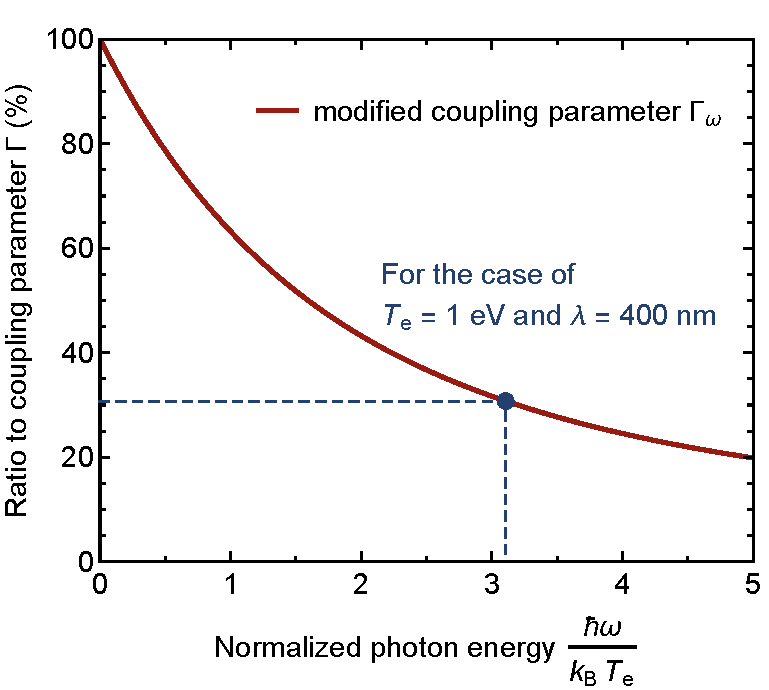
\includegraphics[width=65mm]{figures/ch3/modified/modifiedGamma.pdf}
\caption{The reduction of coupling parameter under the influence of an electromagnetic field. The coupling parameter decreases when the photon energy ``colliding'' to plasma particles is significant.}
\label{fig:modifiedGamma}
\end{figure}

Finally, the thermalization timescale is
\begin{equation}
\tau_{Eei} = \frac{1}{\nu_{Eei}} = \left( \frac{m_i}{m_e} \right) \frac{1}{\nu_{ei}}
\end{equation}
Using the measured data in our experiment \footnote{Plasma produced from argon ($100 \text{ bar}$, room temperature): $T_e \sim 11,000 \text{ K}$ and $n_e \sim 10^{21} \text{ cm}^{-3}$}, the thermalization timescale of electrons and argon ions in the limit of no electric field becomes $\tau_{Eei} \sim 0.2 \text{ ns}$.



%----------------------------------------------------------------------------------------------------
\section{Experimental implementations}
\label{sec:ch3-3}

%----------
\subsection{High-pressure gas discharges}
\label{sec:ch3-3-1}

The strongly coupled plasma that has a high electron density and a relatively low temperature is generated by momentarily depositing energy into a high-pressure gas \cite{tsuda2000calculation, harilal2004spatial, bataller2014blackbody, bataller2016observation}. As an energy source, fs-, ns-lasers, or high voltage sparks are used. The typical lifetime of the plasma Typically, the plasma lasts about a few hundreds of nanoseconds, and the electron temperature and density reach of the order of $1 \text{ eV}$ and $10^{21} \text{ cm}^{-3}$, respectively, achieving $\Gamma \sim 1$. In this experiment, a strong continuous spectrum is usually accompanied at the initial stage of the plasma, and the corresponding signal can be analyzed to diagnose the plasma characteristics. This method guarantees stable repeated experiments because the gas target is quickly restored. Our experiment introduced in Chap.\ref{sec:ch4} also implement high-pressure gas discharge.

%----------
\subsection{Laser-cooled trapped ions}
\label{sec:ch3-3-2}

The application of laser-cooling of ions using either Paul \cite{diedrich1987observation, drewsen1998large} or Penning traps \cite{dubin1999trapped} to generate ultracold neutral plasma by photoionization with additional intense laser is one popular method to create the strongly coupled plasma \cite{murillo2004strongly, langin2019laser, kroker2020ultrafast}. Femtosecond laser provides a precise manipulation of atoms in a Bose-Einstein condensate state, and instantaneous ionization by intense laser pulse realizes the strongly coupled plasma with extremely low temperature with high density. $^{87}$Rb or $^{88}$Sr are the popular elements for such experiments. Plasma generated at a very low temperature seems to have nothing to do with real-world strongly coupled plasma such as the white dwarf stars or the cores of planets at first glance, but in reality, due to the characteristics shared by subjects with similar $\Gamma$, it provides a good research environment for difficult-to-reach targets.

%----------
\subsection{Dusty plasmas}
\label{sec:ch3-3-3}

Dusty plasmas are the classical plasmas containing mesoscopic impurities ranging from a few nanometers to micrometer size, which are the so-called dust grains. Dust grain is considered as an extra species in the plasma to consider in addition to the electrons, ions, and neutral atoms \cite{bellan2008fundamentals}. They are found over a wide range of universe such as interstellar medium \cite{zubko2004interstellar}, protoplanetary disks \cite{pollack1994composition, mcclure2012probing}, Saturn's diffuse E, F, and G rings \cite{goertz1989dusty}, comet tails \cite{davies1997detection}, and noctilucent clouds \cite{havnes1996first}. Generally, the dust grains become highly charged as the electron in-flow toward the mesoscopic particle surface is greater than that of the ion. The surface charge can be of the order of $10^4$ electrons, and the typical number density is about $10^4 \text{ cm}^{-3}$ which leads to the strongly coupled condition for the ``dust grains''. This example is different from the other two introduced previously, that the electrons and ions can be treated with dilute plasma theory, and thus, the Debye shielding is possible for the background plasma, but only the dust particles are strongly correlated by themselves. In our experiment, which will be introduced in Chap.\ref{sec:ch4}, we consider the mesoscopic particles in the plasma where the electrons and ions in the background are in the strongly coupled regime and show how the impurities affect the charge and energy transports in the SCP condition.
